% Copyright 2004 by Till Tantau <tantau@users.sourceforge.net>.
%
% In principle, this file can be redistributed and/or modified under
% the terms of the GNU Public License, version 2.
%
% However, this file is supposed to be a template to be modified
% for your own needs. For this reason, if you use this file as a
% template and not specifically distribute it as part of a another
% package/program, I grant the extra permission to freely copy and
% modify this file as you see fit and even to delete this copyright
% notice. 

\documentclass[xcolor=table]{beamer}
\usepackage{menukeys}[os=win]
\usepackage{textcomp}
\usepackage{tcolorbox}
\usepackage{listings}
\lstset{
  basicstyle=\tiny\ttfamily,
}

% There are many different themes available for Beamer. A comprehensive
% list with examples is given here:
% http://deic.uab.es/~iblanes/beamer_gallery/index_by_theme.html
% You can uncomment the themes below if you would like to use a different
% one:
%\usetheme{AnnArbor}
%\usetheme{Antibes}
%\usetheme{Bergen}
%\usetheme{Berkeley}
%\usetheme{Berlin}
%\usetheme{Boadilla}
%\usetheme{boxes}
%\usetheme{CambridgeUS}
%\usetheme{Copenhagen}
%\usetheme{Darmstadt}
%\usetheme{default}
%\usetheme{Frankfurt}
%\usetheme{Goettingen}
%\usetheme{Hannover}
%\usetheme{Ilmenau}
\usetheme{JuanLesPins}
%\usetheme{Luebeck}
%\usetheme{Madrid}
%\usetheme{Malmoe}
%\usetheme{Marburg}
%\usetheme{Montpellier}
%\usetheme{PaloAlto}
%\usetheme{Pittsburgh}
%\usetheme{Rochester}
%\usetheme{Singapore}
%\usetheme{Szeged}
%\usetheme{Warsaw}
\setbeamerfont{block body}{size=\small}
\title{KF5004 - Primary \texttt{DNS} Server}

% A subtitle is optional and this may be deleted
% \subtitle{(Using proximity detection)}

\author{Dr.~Neil~Eliot\inst{1} / Dr.~Alun~Moon\inst{1}}
% - Give the names in the same order as the appear in the paper.
% - Use the \inst{?} command only if the authors have different
%   affiliation.

%\renewcommand\appendixname{Appendix}

\institute[Northumbria University] % (optional, but mostly needed)
{
  \inst{1}
  Department of Computer and Information Sciences\\
  University of Northumbria
  % \and
  % \inst{2}
  % Department of Theoretical Philosophy\\
  % University of Elsewhere
}
% - Use the \inst command only if there are several affiliations.
% - Keep it simple, no one is interested in your street address.

\date{Session 4}
% - Either use conference name or its abbreviation.
% - Not really informative to the audience, more for people (including
%   yourself) who are reading the slides online

\subject{Introduction}
% This is only inserted into the PDF information catalog. Can be left
% out. 

% If you have a file called "university-logo-filename.xxx", where xxx
% is a graphic format that can be processed by latex or pdflatex,
% resp., then you can add a logo as follows:

% \pgfdeclareimage[height=0.5cm]{university-logo}{university-logo-filename}
% \logo{\pgfuseimage{university-logo}}

% Delete this, if you do not want the table of contents to pop up at
% the beginning of each subsection:
% \AtBeginSubsection[]
% {
%   \begin{frame}<beamer>{Outline}
%     \tableofcontents[currentsection,currentsubsection]
%   \end{frame}
% }

% Let's get started

\begin{document}

\begin{frame}
  \titlepage
\end{frame}

\begin{frame}{Introduction}
  \tableofcontents
  % You might wish to add the option [pausesections]
\end{frame}

% Section and subsections will appear in the presentation overview
% and table of contents.

\section{Introduction to Primary \texttt{DNS}}
\begin{frame}{What is Primary \texttt{DNS} server?}
  \begin{itemize}
    \item A \texttt{Primary DNS} is \texttt{Authoritative} for a \texttt{Zone}.
      \begin{itemize}
          \item \texttt{Zone} $\Longleftrightarrow$ \texttt{Domain}
      \end{itemize}
    \item This server manages the mappings for this zone and the answer will not be derived from anywhere else.
    \item You have spoken directly to the controlling \texttt{Primary server} or its \texttt{Secondary servers}.
  \end{itemize}
  \begin{figure}
    \begin{center}
      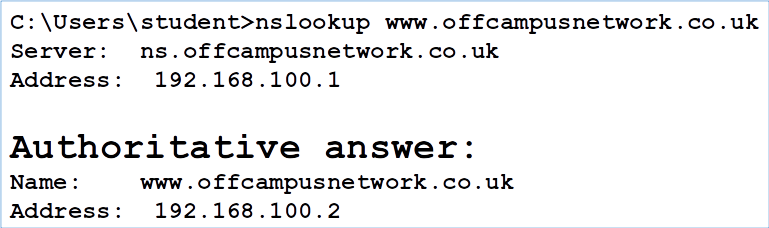
\includegraphics[width=0.8\linewidth]{Authoritative.png}
    \end{center}
  \end{figure}
\end{frame}

\section{Setting up a \texttt{Primary DNS server}}
\subsection{Configuration}
\begin{frame}{Configuring a \texttt{Primary DNS}}
  \begin{itemize}
    \item The configuration of a \texttt{Primary DNS} involves adding a \texttt{zone}.
    \item \texttt{Zones} are ‘pointed to’ from the \texttt{named.conf.local} file.
      \begin{itemize}
        \item \texttt{/etc/bind/named.conf.local}
      \end{itemize}
    \item The config file allows you to specify that the \texttt{zone} is a \texttt{master} and the location of the database.
      \begin{itemize}
        \item The database is a structured text file containing the \texttt{zone} records.
      \end{itemize}
  \end{itemize}
\end{frame}

\begin{frame}[fragile]{Configuring a \texttt{Primary DNS}}
  \lstset{
    basicstyle=\small\ttfamily,
  }
  \begin{lstlisting}
    zone "student.co.uk" {
	    type master;
	    file "/etc/bind/db.student.co.uk";
    };
  \end{lstlisting}
  \begin{tcolorbox}[title={\textbf{NOTE:}}]
    \begin{itemize}
      \item \texttt{/etc/bind/} is the location of \textit{read only} \texttt{zone} files. There will be more on this in \texttt{Advanced OS II} in the final year.
      \item The \texttt{zone} filename standard is \texttt{db.<zone>} e.g. \texttt{db.offcampusnetwork.co.uk} 
    \end{itemize}
  \end{tcolorbox}
\end{frame}

\begin{frame}[fragile]{Configuring a \texttt{Primary DNS}}
  \begin{itemize}
    \item Multiple \texttt{zones} can be declared and managed by one \texttt{DNS} server. 
  \end{itemize}
\lstset{
    basicstyle=\small\ttfamily,
  }
  \begin{lstlisting}
    zone "student.co.uk" {
	    type master;
	    file "/etc/bind/db.student.co.uk";
    };

    zone "staff.co.uk" {
	    type master;
	    file "/etc/bind/db.staff.co.uk";
    };
  \end{lstlisting}
\end{frame}

\subsection{Security}
\begin{frame}{Protecting a \texttt{zone}}
  \begin{itemize}
    \item \texttt{DNS} servers can be used in a \texttt{DDOS} attack.
    \item One technique to prevent this is to limit which machines can use the server.
      \begin{itemize}
        \item \texttt{allow-query\{\};}
      \end{itemize}
    \item All \texttt{zones} can be protected by adding the clause in the \texttt{options} section.  
      \begin{itemize}
        \item \texttt{named.conf.option}
      \end{itemize}
    \item Individual \texttt{zones} can be protected by adding the clause in the \texttt{zone} declaration.  
    \begin{itemize}
      \item \texttt{named.conf.local}
    \end{itemize}
  \end{itemize}
\end{frame}

\begin{frame}{\texttt{A}ccess \texttt{C}ontrol \texttt{L}ists ()\texttt{ACL})}
  \begin{itemize}
    \item Access can be restricted in several ways using an \texttt{ACL}
    \item \texttt{ACL}s can be comma separated lists.
      \begin{itemize}
        \item No security
          \begin{itemize}
            \item \texttt{allow-query\{any;\};}
          \end{itemize}
        \item Individual \texttt{<IP address>}
          \begin{itemize}
            \item \texttt{allow-query\{10.0.0.1;\};}
          \end{itemize}
        \item The network the \texttt{DNS} server resides on.
          \begin{itemize}
            \item \texttt{allow-query\{localnets;\};}
          \end{itemize}
        \item Subnet ranges.
          \begin{itemize}
            \item \texttt{allow-query\{192.168.0.0./16;\};}
          \end{itemize}
        \end{itemize}
  \end{itemize}
\end{frame}

\begin{frame}[fragile]{\texttt{A}ccess \texttt{C}ontrol \texttt{L}ists ()\texttt{ACL})}
  \begin{itemize}
    \item \texttt{ACL} Lists
  \end{itemize}
  \lstset{
    basicstyle=\small\ttfamily,
  }
  \begin{lstlisting}
    allow-query{
      localnets;
      129.168.0.0/16;
      10.0.0.10;
    };
  \end{lstlisting}
\end{frame}

\begin{frame}{\texttt{A}ccess \texttt{C}ontrol \texttt{L}ists ()\texttt{ACL})}
  \begin{itemize}
    \item Any of the options can be reversed by prefixing with an exclamation mark (\texttt{!}).
      \begin{itemize}
        \item Block and individual \texttt{IP}
          \begin{itemize}
            \item \texttt{allow-query\{!10.0.0.1;\};}
          \end{itemize}
        \item Block a subnet ranges.
          \begin{itemize}
            \item \texttt{allow-query\{!192.168.0.0./16;\};}
          \end{itemize}
        \end{itemize}
  \end{itemize}
\end{frame}

\begin{frame}[fragile]{\texttt{A}ccess \texttt{C}ontrol \texttt{L}ists ()\texttt{ACL})}
  \begin{itemize}
    \item \texttt{ACL} Lists in \texttt{named.conf.local}
  \end{itemize}
  \lstset{
    basicstyle=\small\ttfamily,
  }
  \begin{lstlisting}
    zone "student.co.uk" {
      type master;
      file "/etc/bind/db.student.co.uk";
        allow-query{
          localnets;
          10.0.0.0/8;
        };
    };
    
    zone "academics.co.uk" {
      type master;
      file "/etc/bind/db.academics.co.uk";
      allow-query{localnets;};
    };
  \end{lstlisting}
\end{frame}

\subsection{Setting up a \texttt{zone} file}
\begin{frame}{Create a \texttt{zone} file}
  \begin{itemize}
    \item The best way is to copy an existing basic \texttt{zone} file and modify it.
      \begin{itemize}
        \item Fortunately there are a few \texttt{zones} already declared after a default install.
      \end{itemize}
  \item Copy the existing \texttt{db.local} file to create your own \texttt{zone} file.
    \begin{itemize}
      \item e.g. \texttt{\$sudo cp db.local db.student.co.uk}
    \end{itemize}
  \end{itemize}
  \begin{tcolorbox}[title={\textbf{NOTE:}}]
    You require administrative privileges to modify the content of \texttt{/etc/bind} hence using \texttt{sudo}.
  \end{tcolorbox}
\end{frame}

\begin{frame}{Create a \texttt{zone} file}
  \begin{itemize}
    \item Modify the following:
      \begin{itemize}
        \item \texttt{localhost} $\Longrightarrow$ \texttt{<FQDN>}
        \item \texttt{127.0.0.1} $\Longrightarrow$ \texttt{<IP Address of your server>}
        \item \texttt{root.local} $\Longrightarrow$ \texttt{<Your email address>}
          \begin{itemize}
            \item Replace the @ with a . 
            \item e.g. \texttt{i.am@student.co.uk} $\Longrightarrow$ \texttt{i.am.student.co.uk}
          \end{itemize}
      \end{itemize}
  \end{itemize}
  \begin{tcolorbox}[title={\textbf{NOTE:}}]
    \texttt{FQDN} $\equiv$ \texttt{F}ully \texttt{Q}ualified \texttt{D}omain \texttt{N}ame
    \begin{itemize}
      \item e.g. \texttt{student.co.uk.}
    \end{itemize}
  \end{tcolorbox}
\end{frame}

\begin{frame}[fragile]{Create a \texttt{zone} file}
  \begin{itemize}
    \item Assume:
      \begin{itemize}
        \item \texttt{nameserver} is \texttt{ns.student.co.uk}
        \item \texttt{IP} is \texttt{192.168.0.55} (yours will be different)
        \item Admin's email address is \texttt{admin@student.co.uk}
      \end{itemize}
  \end{itemize}
  \begin{itemize}
    \item Default File:
  \end{itemize}
  \lstset{
    basicstyle=\tiny\ttfamily,
  }
  \begin{lstlisting}
;
; BIND data file for local loopback interface
;
$TTL    604800
@   IN    SOA localhost.  root.localhost. (
        2         ; Serial
        604800    ; Refresh
        86400     ; Retry
        2419200   ; Expire
        604800)   ; Negative Cache TTL
;
@   IN    NS    localhost.
@   IN    A     127.0.0.1
@   IN    AAAA  ::1
  \end{lstlisting}
\end{frame}

\begin{frame}[fragile]{Create a \texttt{zone} file}
  \begin{itemize}
    \item Modified File:
  \end{itemize}
  \lstset{
    basicstyle=\tiny\ttfamily,
  }
  \begin{lstlisting}
;
; BIND data file for local loopback interface
;
$ORIGIN student.co.uk.
$TTL    604800
@   IN    SOA student.co.uk.  i.am.student.co.uk. (
        2022012110  ; Serial
        604800      ; Refresh
        86400       ; Retry
        2419200     ; Expire
        604800)     ; Negative Cache TTL
;
@   IN    NS    ns.student.co.uk.
ns  IN    A     192.168.0.55
  \end{lstlisting}
  \begin{tcolorbox}[title={\textbf{NOTE:}}]
    For completeness a few additional changes have been added. These will be discussed later.
  \end{tcolorbox}
\end{frame}

\begin{frame}{Create a \texttt{zone} file}
  \begin{itemize}
    \item Serial Numbers:
      \begin{itemize}
        \item Most administrators like to use the last date edited as the serial of a \texttt{zone}
        \item The format used is \texttt{YYYYMMDDSS} (where \texttt{SS} is a 2 digit sequence number incremented after each edit)
          \begin{itemize}
            \item e.g. \texttt{2020012110}
          \end{itemize}
      \end{itemize}
  \end{itemize}
  \begin{tcolorbox}
    \begin{center}
      \texttt{21\textsuperscript{st} January 2020 Sequence 10}
    \end{center}
  \end{tcolorbox}
\end{frame}

\begin{frame}{Restarting \texttt{BIND9} after a \texttt{zone} change}
  \begin{itemize}
    \item When any changes are made to a \texttt{zone} file the \texttt{BIND9} service must be restarted.
      \begin{itemize}
        \item \texttt{\$sudo systemctl restart bind9}
      \end{itemize}
    \item Restarting the \texttt{daemon} initiates a check of the \texttt{Serial Number} and compiles the database.
  \end{itemize}
  \begin{tcolorbox}[title={\textbf{NOTE:}}]
    Whenever a change is made to a \texttt{zone} file the \texttt{Sequence Number} \textbf{MUST} be updated or the changes will not take place. \texttt{BIND9} \textbf{ONLY} recompiles the database if the \texttt{Sequence Number} is greater than the previously stored value.
  \end{tcolorbox}
\end{frame}

\section{\texttt{Zone} Files}
\subsection{\texttt{Format}}
\begin{frame}{\texttt{Zone} File Format}
  \begin{itemize}
    \item \texttt{Zone} files are text files (standardized by \texttt{RFC 1035})
      \begin{itemize}
        \item As such they can be edited with any standard text editor.
      \end{itemize}
    \item They consist of three entry types:
      \begin{itemize}
        \item \texttt{Comments}
        \item \texttt{Directives}
        \item \texttt{Resource Records} (\texttt{RR})
      \end{itemize}
  \end{itemize}
  \begin{tcolorbox}[title={\textbf{NOTE:}}]
    In this module we will only be covering a subset of the \texttt{Directives} and \texttt{Resource Records}.
  \end{tcolorbox}  
\end{frame}

\begin{frame}{\texttt{Zone} File Format}
  \begin{itemize}
    \item \texttt{Comments:} All comments start with a semicolon (;) and continue to the end of the line. 
      \begin{itemize}
        \item \texttt{Comments} can be added to any other record type and are assumed to terminate the line.
      \end{itemize}
    \item \texttt{Directives:} All \texttt{directives} start with a dollar sign (\texttt{\$}) and are used to control processing of the \texttt{zone} files.
    \item \texttt{Resource Record}s: Are used to define the characteristics, properties, or entities contained within the \texttt{domain}. 
    \begin{itemize}
        \item \texttt{RR}s are contained on a single line or spread across multiple lines by enclosing the sub-components in parentheses. i.e. the \texttt{SOA} record.
      \end{itemize}
  \end{itemize}
\end{frame}

\begin{frame}[fragile]{\texttt{Zone} File Format}
  \lstset{
    basicstyle=\scriptsize\ttfamily,
  }
  \begin{lstlisting}
; this is a full line comment
$TTL 12h ; directive - comment terminates the line
$ORIGIN example.com.
; Start of Authority (SOA) record defining the zone (domain)
; illustrates an RR record spread over more than one line
; using the enclosing parentheses
@     IN    SOA   example.com.  hostmaster.example.com. (
        2020010101 ; se = serial number
        3h ; ref = refresh
        15m ; ret = update retry
        3w ; ex = expiry
        2h20m ; min = minimum
        )
    ; single line RR
@	    IN    NS    ns1.example.com.
ns1   IN    A     192.168.0.99
  \end{lstlisting}
\end{frame}

\begin{frame}{\texttt{Zone} File Format (Directives)}
  \begin{itemize}
    \item \texttt{\$TTL}
      \begin{itemize}
        \item Defines the default \texttt{TTL} (\texttt{T}ime \texttt{T}o \texttt{L}ive) value for the \texttt{zone}, which is the time a \texttt{RR} may be cached by another \texttt{DNS} server.
        \item This directive is \textbf{mandatory}.
      \end{itemize}
      \item \texttt{\$ORIGIN}
      \begin{itemize}
        \item Declares the \texttt{domain name} for the \texttt{zone} being defined.
        \item This directive is \textbf{optional}.
        \begin{itemize} 
          \item \textbf{You should always use it – default behaviours can change!)}.
        \end{itemize}
      \end{itemize}
  \end{itemize}
\end{frame}

\begin{frame}{\texttt{Zone} File Format (Directives)}
  \begin{itemize}
    \item \texttt{\$SOA} (\texttt{S}tart \texttt{O}f \texttt{A}uthority)
       \begin{itemize}
         \item It describes the global characteristics of the \texttt{zone}.
         \item There can be only one \texttt{SOA RR} in a \texttt{zone} file. 
         \item The \texttt{SOA RR} \textbf{must} appear as the first \texttt{RR} in a \texttt{zone} file and is therefore \textbf{mandatory}.
       \end{itemize}
     \item \texttt{\$NS} (\texttt{N}ame \texttt{S}erver)
       \begin{itemize}
         \item Defines \texttt{name servers} that are authoritative for the \texttt{zone}. 
         \item There should be one or more \texttt{NS RR}s in a \texttt{zone} 
           \begin{itemize}
             \item Why?
           \end{itemize} 
         \item \texttt{NS RR}s may reference servers in this \texttt{zone} or an external \texttt{zone}. 
         \item This directive is \textbf{mandatory}.
       \end{itemize}
  \end{itemize}
\end{frame}

\begin{frame}{\texttt{Zone} File Format (Directives)}
  \begin{itemize}
    \item \texttt{\$MX} (\texttt{M}ail E\texttt{X}changer)
       \begin{itemize}
          \item Defines the mail servers for the \texttt{zone}. 
          \item There may be zero or more \texttt{MX RR}s in a \texttt{zone} file.
            \begin{itemize}
              \item If the \texttt{domain} does not provide e-mail services there is no need for any \texttt{MX RR}s.
            \end{itemize} 
         \item An \texttt{MX RR} may reference a mail server in this \texttt{domain} or in an external \texttt{domain}. 
         \item This directive is \textbf{optional}.
       \end{itemize}
  \end{itemize}
\end{frame}

\begin{frame}{\texttt{Zone} File Format (Directives)}
  \begin{itemize}
    \item \texttt{\$A} (\texttt{A}ddress)
       \begin{itemize}
          \item Used to define the \texttt{IPv4} address of all the hosts (or services) in the \texttt{zone}.
          \item This directive is \textbf{optional}.
       \end{itemize}
  \end{itemize}
  \begin{tcolorbox}
    \begin{center}
      \texttt{nslookup -type=A www.google.com}\\
      \texttt{nslookup -type=A www.google.com.}
    \end{center}
  \end{tcolorbox}
  \begin{tcolorbox}[title={\textbf{NOTE:}}]
      An \texttt{FQDN} should have the period (.) at the end. The period signifies the \texttt{root} of the global \texttt{DNS} system.
  \end{tcolorbox}
\end{frame}

\begin{frame}{\texttt{Zone} File Format (Directives)}
  \begin{itemize}
    \item \texttt{\$AAAA} (\texttt{A}ddress)
       \begin{itemize}
          \item Used to define the \texttt{IPv6} address of all the hosts (or services) in the \texttt{zone}.
          \item This directive is \textbf{optional}.
       \end{itemize}
  \end{itemize}
  \begin{tcolorbox}
    \begin{center}
      \texttt{nslookup -type=AAAA www.google.com}\\
      \texttt{nslookup -type=AAAA www.google.com.}
    \end{center}
  \end{tcolorbox}
  \begin{tcolorbox}[title={\textbf{NOTE:}}]
      The \texttt{AAAA} directive is not used in the module.
  \end{tcolorbox}
\end{frame}

\begin{frame}{\texttt{Zone} File Format (Directives)}
  \begin{itemize}
    \item \texttt{\$CNAME} (\texttt{C}anonical \texttt{N}ame)
       \begin{itemize}
          \item Used to define an alias for another \texttt{A} or \texttt{AAAA} \texttt{RR}.
          \item This directive is \textbf{optional}.
       \end{itemize}
  \end{itemize}
\end{frame}

\begin{frame}[fragile]{\texttt{Zone} File Format}
  \lstset{
    basicstyle=\scriptsize\ttfamily,
  }
  \begin{lstlisting}
; this is a full line comment
$TTL 12h ; directive - comment terminates the line
$ORIGIN example.com.
; Start of Authority (SOA) record defining the zone (domain)
; illustrates an RR record spread over more than one line
; using the enclosing parentheses
@         IN      SOA  example.com.  hostmaster.example.com. (
          2020010101 ; se = serial number
          3h ; ref = refresh
          15m ; ret = update retry
          3w ; ex = expiry
          2h20m ; min = minimum
        )
; single line RR’s
          IN      NS            ns1.example.com.
      3w  IN      MX      10    mail.example.com.
ns1       IN      A             192.168.254.2
mail      IN      A             192.168.254.4
www       IN      A             192.168.254.7
M1        IN	  AAAA          2001:db8::1
  \end{lstlisting}
\end{frame}

\subsection{Tailoring the \texttt{Zone}}
\begin{frame}{\texttt{Directive} effects}
  \begin{itemize}
    \item \texttt{\$TTL} (\texttt{T}ime \texttt{T}o \texttt{L}ive)
       \begin{itemize}
          \item Every \texttt{RR} has an optional \texttt{TTL} value which is defined, by default in seconds.
          \item The \texttt{\$TTL} directive is standardized in \texttt{RFC 2308} and defines the default \texttt{TTL} value applied to any \texttt{RR} that does not have an explicit \texttt{TTL} defined. 
          \item \texttt{TTL}, in the context of \texttt{DNS}, defines the time in seconds that a record may be cached by another \texttt{name server} or a \texttt{resolver}.
       \end{itemize}
    \item Syntax
       \begin{itemize}
          \item \texttt{\$TTL time-in-seconds}
          \item e.g. \texttt{\$TTL} 172800
          \item e.g. \texttt{\$TTL} 2d
       \end{itemize}
  \end{itemize}
\end{frame}

\begin{frame}{\texttt{Directive} effects}
  \begin{tcolorbox}[title={\textbf{NOTE:}}]
    Although not defined in the \texttt{RFC} standard it is common practice to use alternative notations to just using seconds.
    \begin{itemize}
      \item \texttt{m}=month
      \item \texttt{w}=week
      \item \texttt{d}=days
      \item \texttt{s}=seconds
    \end{itemize}
    e.g. \texttt{\$TTL} 2d
  \end{tcolorbox}
\end{frame}

\begin{frame}{\texttt{Directive} effects}
  \begin{itemize}
    \item \texttt{\$TTL}
      \begin{itemize}
        \item \texttt{0} indicates never cache the record.
          \begin{itemize}
            \item Useful?
          \end{itemize}
        \item \texttt{2147483647} - max, which is over 68 years
          \begin{itemize}
            \item Dangerous?
          \end{itemize}
      \end{itemize}
  \end{itemize}
  \begin{tcolorbox}[title={\textbf{NOTE:}}]
    The current best practice recommendations (\texttt{RFC 1912}) state that \texttt{RR}s that rarely change should be considered for multi-week values.
  \end{tcolorbox}
\end{frame}

\begin{frame}{\texttt{Directive} effects}
  \begin{itemize}
    \item \texttt{\$ORIGIN}
      \begin{itemize}
        \item Standardised in \texttt{RFC 1035}, it defines the \texttt{domain name} that will be appended to any incomplete \texttt{names/labels} in the \texttt{zone} file (sometimes called an unqualified name).
        \item This process reduces the amount of work required to define machine names and addresses in \texttt{RR}.
        \item This process of appending to names that do not end with a dot can be a major source of \texttt{zone} file configuration errors.
      \end{itemize}
  \end{itemize}
  \begin{tcolorbox}[title={\textbf{NOTE:}}]
    Currently \texttt{BIND9} uses the \texttt{zone} declaration for ths purpose. However that may changes so it should be used to comply with current practice. Also other \texttt{DNS} software may not use that approach.
  \end{tcolorbox}
\end{frame}

\begin{frame}{\texttt{\$Directive} effects}
  \begin{itemize}
    \item \texttt{\$ORIGIN} Substitution rule:
      \begin{itemize}
        \item If a name appears in a \texttt{RR} and does not end with a dot then the value of the last or only \texttt{\$ORIGIN} directive will be appended to the name.
        \item If the name ends with a dot, then it is an \texttt{FQDN} and nothing will be appended.
      \end{itemize}
  \end{itemize}
  \begin{tcolorbox}[title={\textbf{NOTE:}}]
    \texttt{\$ORIGIN} can appear in a \texttt{zone} file more than once and is used to great effect when implementing \texttt{sub-domains} (More on that later!).
  \end{tcolorbox}
\end{frame}

\section{Implementation}
\subsection{Directives effects}
\begin{frame}{\texttt{\$ORIGIN}}
  \begin{itemize}
    \item Syntax:
      \begin{itemize}
        \item \texttt{\$ORIGIN domain-name}
      \end{itemize}
  \end{itemize}
  \begin{tcolorbox}
    \begin{center}
      \texttt{\$ORIGIN example.com.}      
    \end{center}
  \end{tcolorbox}
\end{frame}

\subsection{\texttt{RR}}
\begin{frame}[fragile]{\texttt{SOA}}
  \begin{itemize}
    \item Syntax:
      \begin{itemize}
        \item \texttt{name ttl class rr name-server e-mail sn refresh retry expiry min}
      \end{itemize}
  \end{itemize}
  \begin{tcolorbox}
    \lstset{
      basicstyle=\scriptsize\ttfamily,
    }
    \begin{lstlisting}
@   IN  SOA  example.com.  hostmaster.example.com. (
        2020010101 ; se = serial number
        3h ; ref = refresh
        15m ; ret = update retry
        3w ; ex = expiry
        2h20m ; min = minimum
)
    \end{lstlisting}
    \end{tcolorbox}
\end{frame}

\begin{frame}{\texttt{SOA}}
  \begin{table}
    \rowcolors{1}{}{lightgray} %-- this indicates the change in odd and pair rows
    \tiny
    \begin{tabular}{|p{1.6cm}|p{1.6cm}|p{4.7cm}|} 
      \hline
      \rowcolor{gray}
      \multicolumn{1}{|c|}{Syntax} & \multicolumn{1}{c|}{Example} & \multicolumn{1}{c|}{Description}\\ 
      \hline
      \texttt{name}&@&The \texttt{@} symbol substitutes the current value of \texttt{\$ORIGIN} (in the example file this is example.com.).\\
      \hline
      \texttt{ttl}&&There is no \texttt{ttl} value defined for the \texttt{RR} (in this case), so the zone default of \texttt{2d} (172800 seconds) from the \texttt{\$TTL} directive will be used.\\
      \hline
      \texttt{class}&\texttt{IN}&\texttt{IN} defines the class to be Internet (defaulted if omitted). Other values exist but are rarely used.\\
      \hline
      \texttt{name-server}&\texttt{ns1.example.com.}&Defines the \texttt{Primary Master} name server for the zone and has a special meaning only when used with \texttt{Dynamic DNS} configurations\\
      \hline
      \texttt{e-mail}&\texttt{ad@example.com.}&Defines an administrative \texttt{e-mail} address for the zone. It is recommended in \texttt{RFC 2142} that the \texttt{e-mail} address hostmaster be used uniquely for this purpose\\
      \hline
      \texttt{sn}&\texttt{2020010101}&Defines the serial number currently associated with the zone. The serial number must be updated every time any change is made to the domain. (usually using a date format?)\\
      \hline
    \end{tabular}
  \end{table}
  continued...
\end{frame}

\begin{frame}{\texttt{SOA}}
  \begin{table}
    \rowcolors{1}{}{lightgray} %-- this indicates the change in odd and pair rows
    \tiny
    \begin{tabular}{|p{1.6cm}|p{1.6cm}|p{4.7cm}|} 
      \hline
      \rowcolor{gray}
      \multicolumn{1}{|c|}{Syntax} & \multicolumn{1}{c|}{Example} & \multicolumn{1}{c|}{Description}\\ 
      \hline
      \texttt{refresh}&\texttt{12h}&When the refresh value is reached, the slave name server for this zone will try to read the \texttt{SOA RR} from the zone master.\\
      \hline
      \texttt{retry}&\texttt{15m}&Defines the retry interval in seconds if the \texttt{slave} fails to make contact with the zone master during a refresh cycle\\
      \hline
      \texttt{expire}&\texttt{3w}&Defines the time in seconds after which the \texttt{zone} records are assumed to be no longer authoritative. \texttt{BIND} interprets this to mean that the records can no longer be considered valid and consequentially stops responding to queries for the zone.\\
      \hline
      \texttt{nx}&\texttt{3h}&\texttt{nx} was redefined in \texttt{RFC 2308} to be the period of time that negative responses can be cached by a \texttt{resolver}.\\
      \hline
    \end{tabular}
  \end{table}
\end{frame}

\begin{frame}{\texttt{NS}}
  \begin{itemize}
      \item The \texttt{NS RR} is standardized in \texttt{RFC 1035} and defines the authoritative \texttt{name servers} (there should be at least two) for the \texttt{domain}.
      \item A \texttt{NS} record tells \texttt{name servers} which machines are in charge of a given \texttt{domain}. This has one data-dependent field: The name of the \texttt{DNS} node which a given \texttt{NS} record points to. 
  \end{itemize}
\end{frame}

\begin{frame}{\texttt{NS}}
  \begin{itemize}
    \item Syntax
      \begin{itemize}
        \item \texttt{name ttl class rr name}
      \end{itemize}
    \item e.g.
      \begin{itemize}
        \item \texttt{ IN NS ns1.example.com.}
      \end{itemize}
  \end{itemize}
\end{frame}

\begin{frame}{\texttt{NS}}
  \begin{table}
    \rowcolors{1}{}{lightgray} %-- this indicates the change in odd and pair rows
    \tiny
    \begin{tabular}{|p{1.6cm}|p{1.6cm}|p{4.7cm}|} 
      \hline
      \rowcolor{gray}
      \multicolumn{1}{|c|}{Syntax} & \multicolumn{1}{c|}{Example} & \multicolumn{1}{c|}{Description}\\ 
      \hline
      \texttt{name}&&This field is blank (may be either a space or a tab character) it is implicitly substituted with the current value of the name. You could also write this record as \texttt{example.com.} \texttt{IN NS ns1.example.com.}\\
      \hline
      \texttt{ttl}&&There is no \texttt{ttl} value defined for the \texttt{RR}, so the \texttt{zone} default from the \texttt{\$TTL} directive will be used.\\
      \hline
      \texttt{class}&\texttt{IN}&Internet Class.\\
      \hline
      \texttt{name}&\texttt{ns1.example.com.}&Defines a \texttt{name server} that is authoritative for the \texttt{domain}. In this example, an \texttt{FQDN} format has been used, but it could have been
      written as just \texttt{ns1} (without the dot) and \texttt{\$ORIGIN} substitution would take place. This \texttt{NS} record points to a \texttt{name server} within the \texttt{domain} and therefore there \texttt{MUST} be a corresponding \texttt{A RR} for \texttt{IPv4} (or \texttt{AAAA RR}
      if \texttt{IPv6}) defined.\\
      \hline
    \end{tabular}
  \end{table}
\end{frame}

\begin{frame}{\texttt{MX}}
  \begin{itemize}
      \item The \texttt{MX RR} is standardized in \texttt{RFC 1035} and defines the mail server(s) (mail exchangers) for the \texttt{domain}.
  \end{itemize}
\end{frame}

\begin{frame}{\texttt{MX}}
  \begin{itemize}
    \item Syntax
      \begin{itemize}
        \item \texttt{name ttl class rr preference name}
      \end{itemize}
    \item e.g.
      \begin{itemize}
        \item \texttt{ 3w IN MX mail.example.com.}
      \end{itemize}
  \end{itemize}
\end{frame}

\begin{frame}{\texttt{MS}}
  \begin{table}
    \rowcolors{1}{}{lightgray} %-- this indicates the change in odd and pair rows
    \tiny
    \begin{tabular}{|p{1.6cm}|p{1.6cm}|p{4.7cm}|} 
      \hline
      \rowcolor{gray}
      \multicolumn{1}{|c|}{Syntax} & \multicolumn{1}{c|}{Example} & \multicolumn{1}{c|}{Description}\\ 
      \hline
      \texttt{name}&&This field is blank and implicitly substitutes the value of the right hand name field from the previous \texttt{RR} (in the example file, this is \texttt{example.com.}).\\
      \hline
      \texttt{ttl}&3w&This illustrates the use of an explicit \texttt{ttl} value in a \texttt{RR} that overrides the \texttt{zone} default (defined in the \texttt{\$TTL} directive). The value shown (three weeks) is significantly higher than the example \texttt{zone} default, which is two days. This is because the \texttt{domain MX RR} is unlikely to change (its corresponding \texttt{A RR} may change more frequently).\\
      \hline
      \texttt{class}&\texttt{IN}&Internet Class.\\
      \hline
      \texttt{name}&\texttt{ns1.example.com.}&Defines a \texttt{name server} that is authoritative for the \texttt{domain}. In this example, an \texttt{FQDN} format has been used, but it could have been written as just \texttt{ns1} (without the dot) and \texttt{\$ORIGIN} substitution would take place. This \texttt{NS} record points to a \texttt{name server} within the \texttt{domain} and therefore there \texttt{MUST} be a corresponding \texttt{A RR} for \texttt{IPv4} (or \texttt{AAAA RR} if \texttt{IPv6}) defined.\\
      \hline
    \end{tabular}
  \end{table}
  Continued...
\end{frame}

\begin{frame}{\texttt{MS}}
  \begin{table}
    \rowcolors{1}{}{lightgray} %-- this indicates the change in odd and pair rows
    \tiny
    \begin{tabular}{|p{1.6cm}|p{1.7cm}|p{4.7cm}|} 
      \hline
      \rowcolor{gray}
      \multicolumn{1}{|c|}{Syntax} & \multicolumn{1}{c|}{Example} & \multicolumn{1}{c|}{Description}\\ 
      \hline
      \texttt{name}&\texttt{mail.example.com.}&Defines a mail server with the defined \texttt{preference} value for the \texttt{domain}. In this example, an \texttt{FQDN} format has been used, but you could write this as just \texttt{mail} if it is in the same \texttt{zone}.\\
      \hline
    \end{tabular}
  \end{table}
\end{frame}

\begin{frame}{\texttt{A}}
  \begin{itemize}
      \item The \texttt{A RR} is standardized in \texttt{RFC 1035} and defines the \texttt{IPv4} address of a particular host in the \texttt{zone}.
  \end{itemize}
\end{frame}

\begin{frame}{\texttt{A}}
  \begin{itemize}
    \item Syntax
      \begin{itemize}
        \item \texttt{name ttl class rr ipv4}
      \end{itemize}
    \item e.g.
      \begin{itemize}
        \item \texttt{www ~IN A 192.168.254.7}
        \item \texttt{mail IN A 192.168.254.4}
      \end{itemize}
  \end{itemize}
\end{frame}

\begin{frame}{\texttt{A}}
  \begin{table}
    \rowcolors{1}{}{lightgray} %-- this indicates the change in odd and pair rows
    \tiny
    \begin{tabular}{|p{1.6cm}|p{1.6cm}|p{4.7cm}|} 
      \hline
      \rowcolor{gray}
      \multicolumn{1}{|c|}{Syntax} & \multicolumn{1}{c|}{Example} & \multicolumn{1}{c|}{Description}\\ 
      \hline
      \texttt{name}&www&The name is unqualified, causing \texttt{\$ORIGIN} substitution. You could write this as \texttt{www.example.com.}\\
      \hline
      \texttt{ttl}&&There is no \texttt{ttl} value defined for the \texttt{RR}, so the \texttt{zone} default from the \texttt{\$TTL} directive will be used. (0 would prevent caching!)\\
      \hline
      \texttt{class}&\texttt{IN}&Internet Class.\\
      \hline
      \texttt{ipv4}&\texttt{192.168.254.7}&Defines that the host \texttt{www} has the physical \texttt{IPv4} address \texttt{192.168.254.7}. Records defined by \texttt{NS} or \texttt{MX RR}s that have \texttt{name}s contained within the \texttt{domain} \textbf{MUST} have corresponding \texttt{A RR}.\\
      \hline
    \end{tabular}
  \end{table}
\end{frame}

\begin{frame}{\texttt{CNAME}}
  \begin{itemize}
      \item The \texttt{CNAME RR} is standardized in \texttt{RFC 1035} and defines an alias for an existing host defined by an \texttt{A} or \texttt{AAAA RR}.
  \end{itemize}
\end{frame}

\begin{frame}{\texttt{CNAME}}
  \begin{itemize}
    \item Syntax
      \begin{itemize}
        \item \texttt{name ttl class rr canonical-name}
      \end{itemize}
    \item e.g.
      \begin{itemize}
        \item \texttt{www ~IN CNAME server.example.com.}
        \item \texttt{mail IN CNAME server.example.com.}
      \end{itemize}
  \end{itemize}
\end{frame}

\begin{frame}{\texttt{CNAME}}
  \begin{table}
    \rowcolors{1}{}{lightgray} %-- this indicates the change in odd and pair rows
    \tiny
    \begin{tabular}{|p{1.6cm}|p{1.9cm}|p{4.7cm}|} 
      \hline
      \rowcolor{gray}
      \multicolumn{1}{|c|}{Syntax} & \multicolumn{1}{c|}{Example} & \multicolumn{1}{c|}{Description}\\ 
      \hline
      \texttt{name}&www&The name is unqualified, causing \texttt{\$ORIGIN} substitution. You could write this as \texttt{www.example.com.}\\
      \hline
      \texttt{ttl}&&There is no \texttt{ttl} value defined for the \texttt{RR}, so the \texttt{zone} default from the \texttt{\$TTL} directive will be used. (0 would prevent caching!)\\
      \hline
      \texttt{class}&\texttt{IN}&Internet Class.\\
      \hline
      \texttt{cannonical-name}&\texttt{server.example.com.}&Defines that the \texttt{name www.example.com} is aliased to the host \texttt{server.example.com.}\\
      \hline
    \end{tabular}
  \end{table}
\end{frame}

\begin{frame}[fragile]{\texttt{CNAME} Issues}
  \begin{itemize}
    \item \texttt{CNAME RR}s are often used when assigning service names to existing hosts.
    \item If a host is actually called \texttt{server} but runs specific services e.g. \texttt{ftp} or \texttt{www}, then \texttt{CNAME RR}s are frequently used to define these services.
  \end{itemize}
  \begin{tcolorbox}
    \lstset{
      basicstyle=\scriptsize\ttfamily,
    }
    \begin{lstlisting}
      ftp     IN CNAME server
      www     IN CNAME server
      server  IN A     192.168.254.21
    \end{lstlisting}
  \end{tcolorbox}
\end{frame}

\begin{frame}[fragile]{\texttt{CNAME} Issues}
  \begin{itemize}
    \item \texttt{CNAME} records should not be used with either \texttt{NS} or \texttt{MX} records.
    \item It is permissable but considered very bad pratice to chain \texttt{CNAME} records.
  \end{itemize}
  \begin{tcolorbox}
    \lstset{
      basicstyle=\scriptsize\ttfamily,
    }
    \begin{lstlisting}
      ftp     IN CNAME www
      www     IN CNAME server
      server  IN A     192.168.254.21
    \end{lstlisting}
  \end{tcolorbox}
\end{frame}

\subsection{Error Checking}
\begin{frame}{\texttt{named-checkzone}}
  \begin{itemize}
    \item The syntax for a \texttt{zone} file can become quite complex and on occasions errors are made.
    \item There is a utility which will validate a \texttt{zone} file.
      \begin{itemize}
        \item \texttt{named-checkzone}.
      \end{itemize}
    \item Syntax:
      \begin{itemize}
        \item \texttt{named-checkzone <domain> <zone file>}.
      \end{itemize}
  \end{itemize}
\end{frame}

\begin{frame}[fragile]{\texttt{named-checkzone}}
  \begin{tcolorbox}
    \lstset{
      basicstyle=\tiny\ttfamily,
    }
    \begin{lstlisting}
student@A1:~$ named-checkzone student.co.uk db.student.co.uk
zone student.co.uk/IN: loaded serial 2020010101
OK
student@A1:~$
    \end{lstlisting}
  \end{tcolorbox}
\end{frame}

\section*{Conclusion}
\begin{frame}{Conclusion}
  \begin{itemize}
    \item What is a \texttt{Primary DNS}?
    \item What is a \texttt{Primary DNS}’s main function?
    \item What is an \texttt{Authoritative DNS} Lookup?
    \item How can you protect a \texttt{zone} from becoming a part of a \texttt{DDOS} attack?
    \item How can you check \texttt{zone} files for errors?
  \end{itemize}
\end{frame}

\end{document}


